% !TEX root =  master.tex
\chapter{Machine Learning Modeling}

\begin{figure}[hbtp]
    \centering
    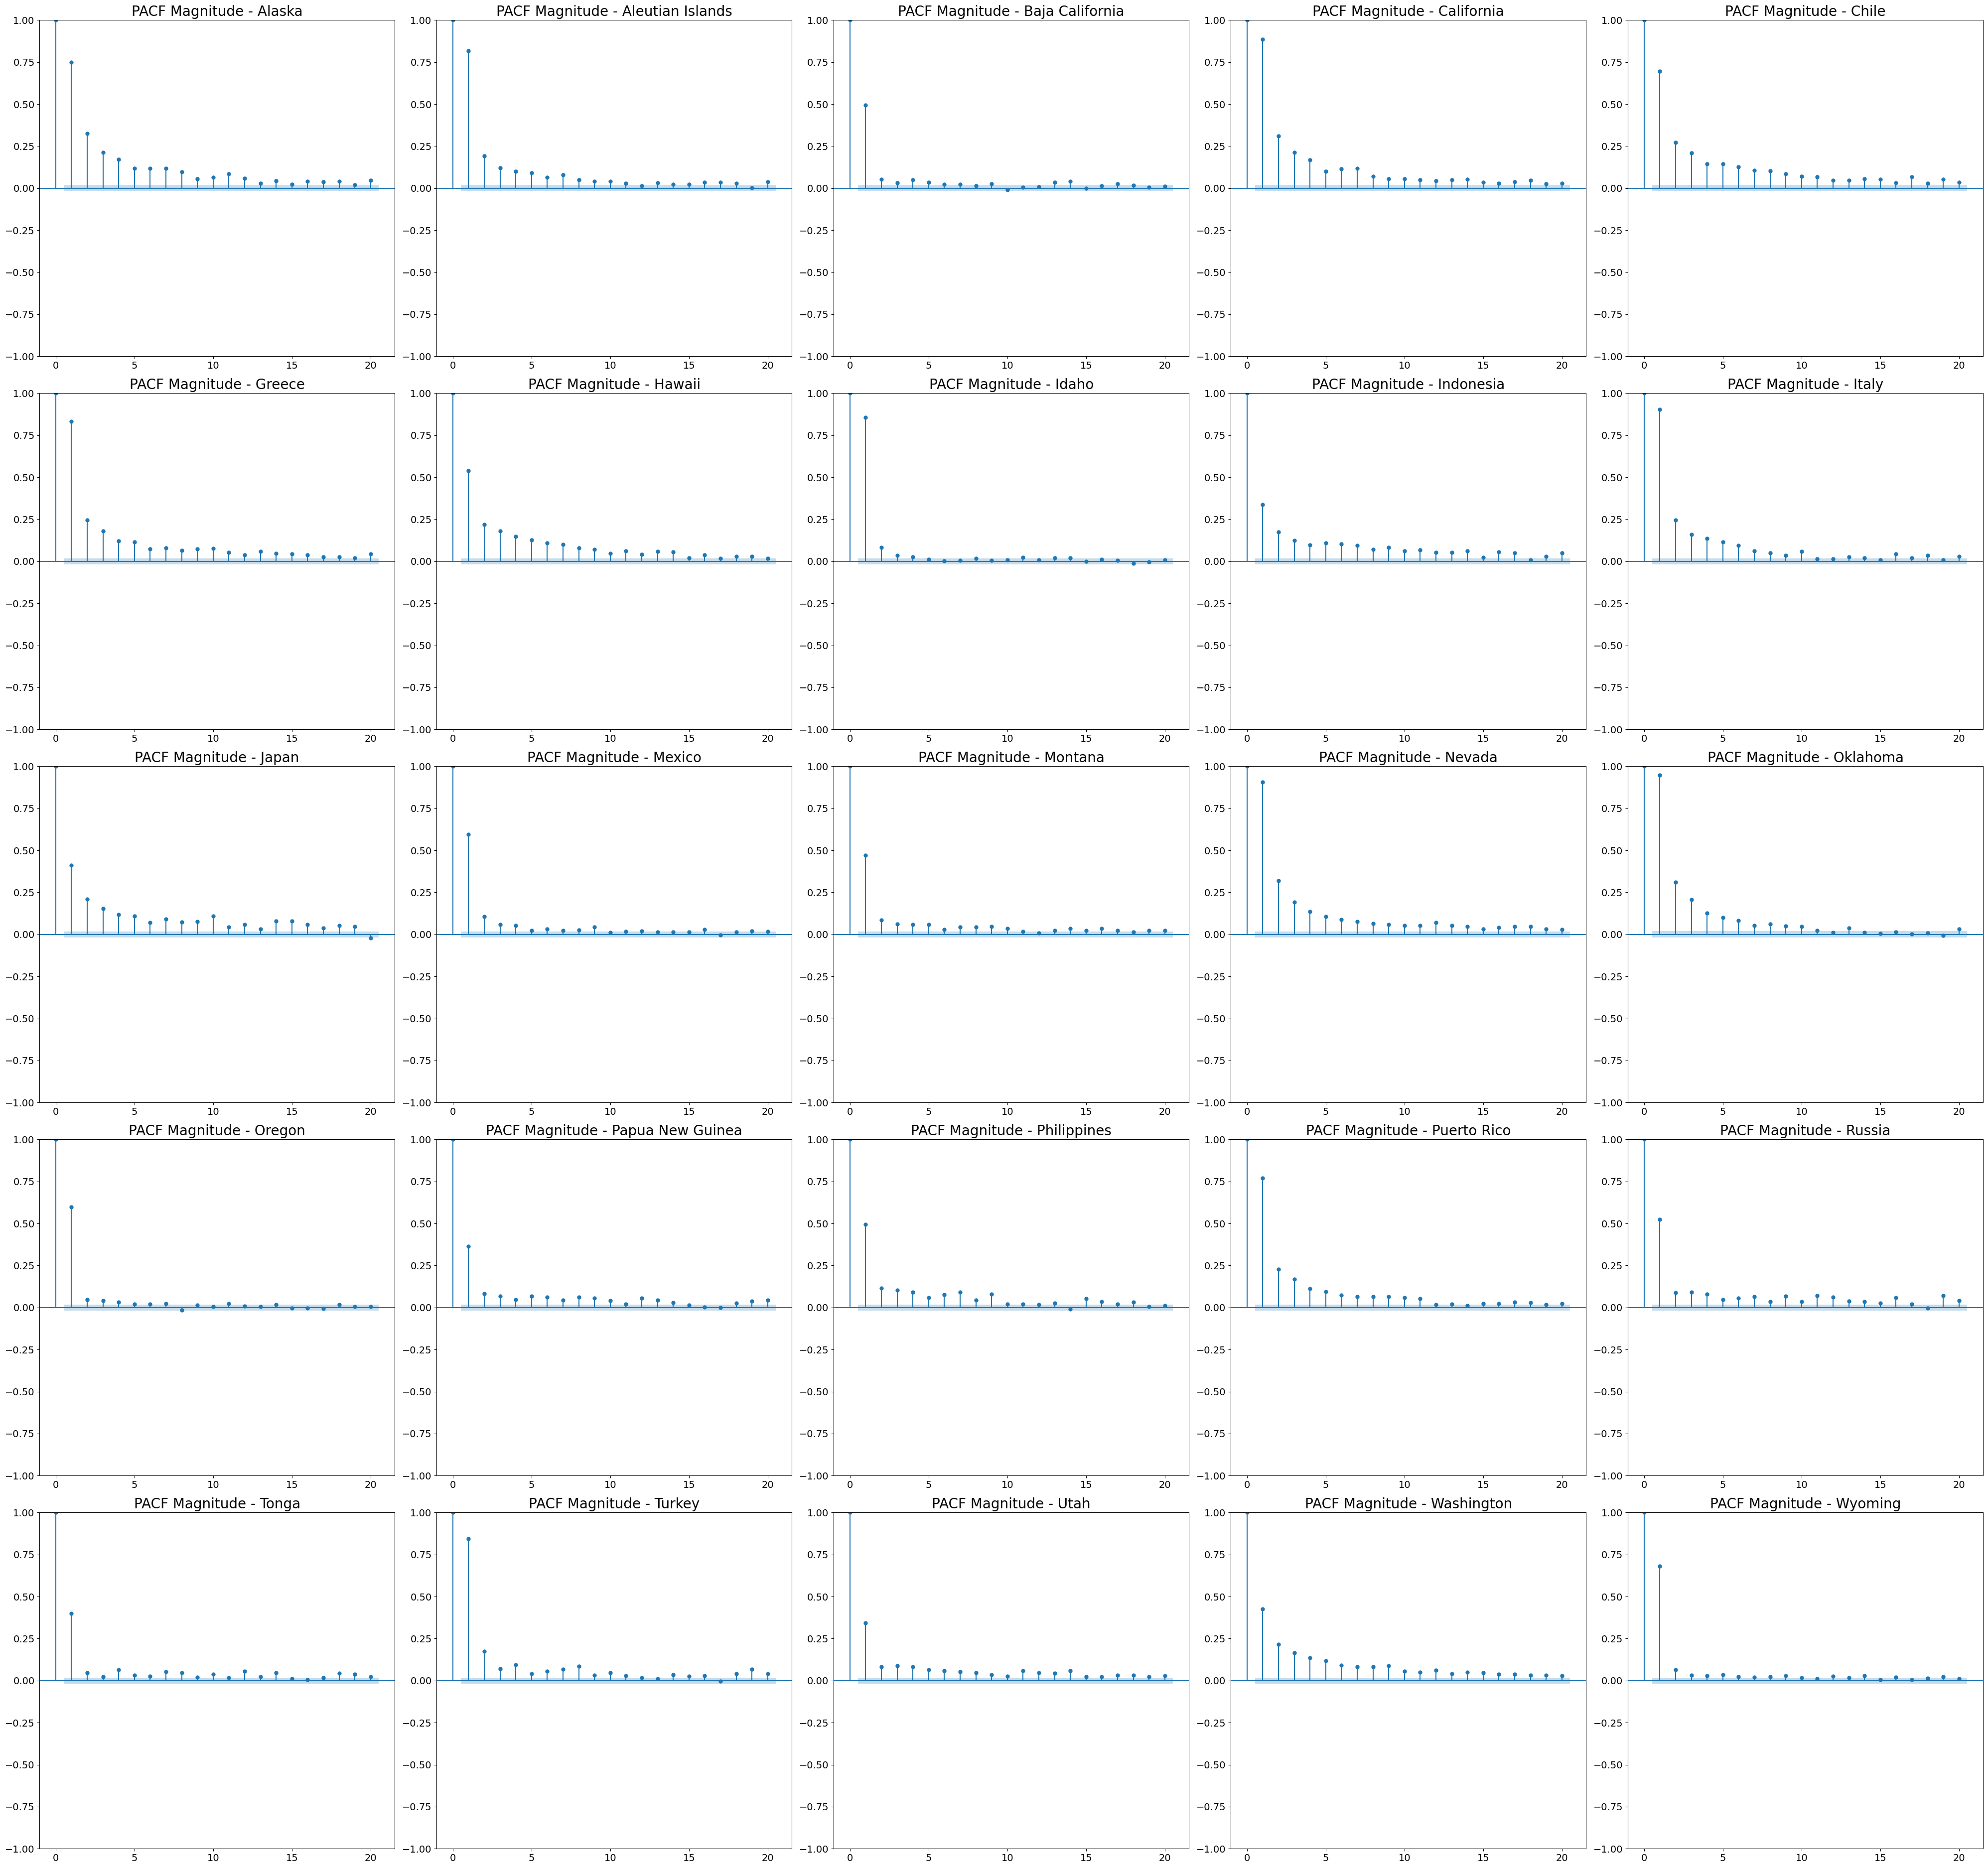
\includegraphics[scale=0.15]{img/magnitude-pacf-per-region.png}
    \captionsetup{format=hang}
    \caption{\label{fig:mag-pacf}Magnitude partial autocorrelation per region.}
\end{figure}

\begin{figure}[hbtp]
    \centering
    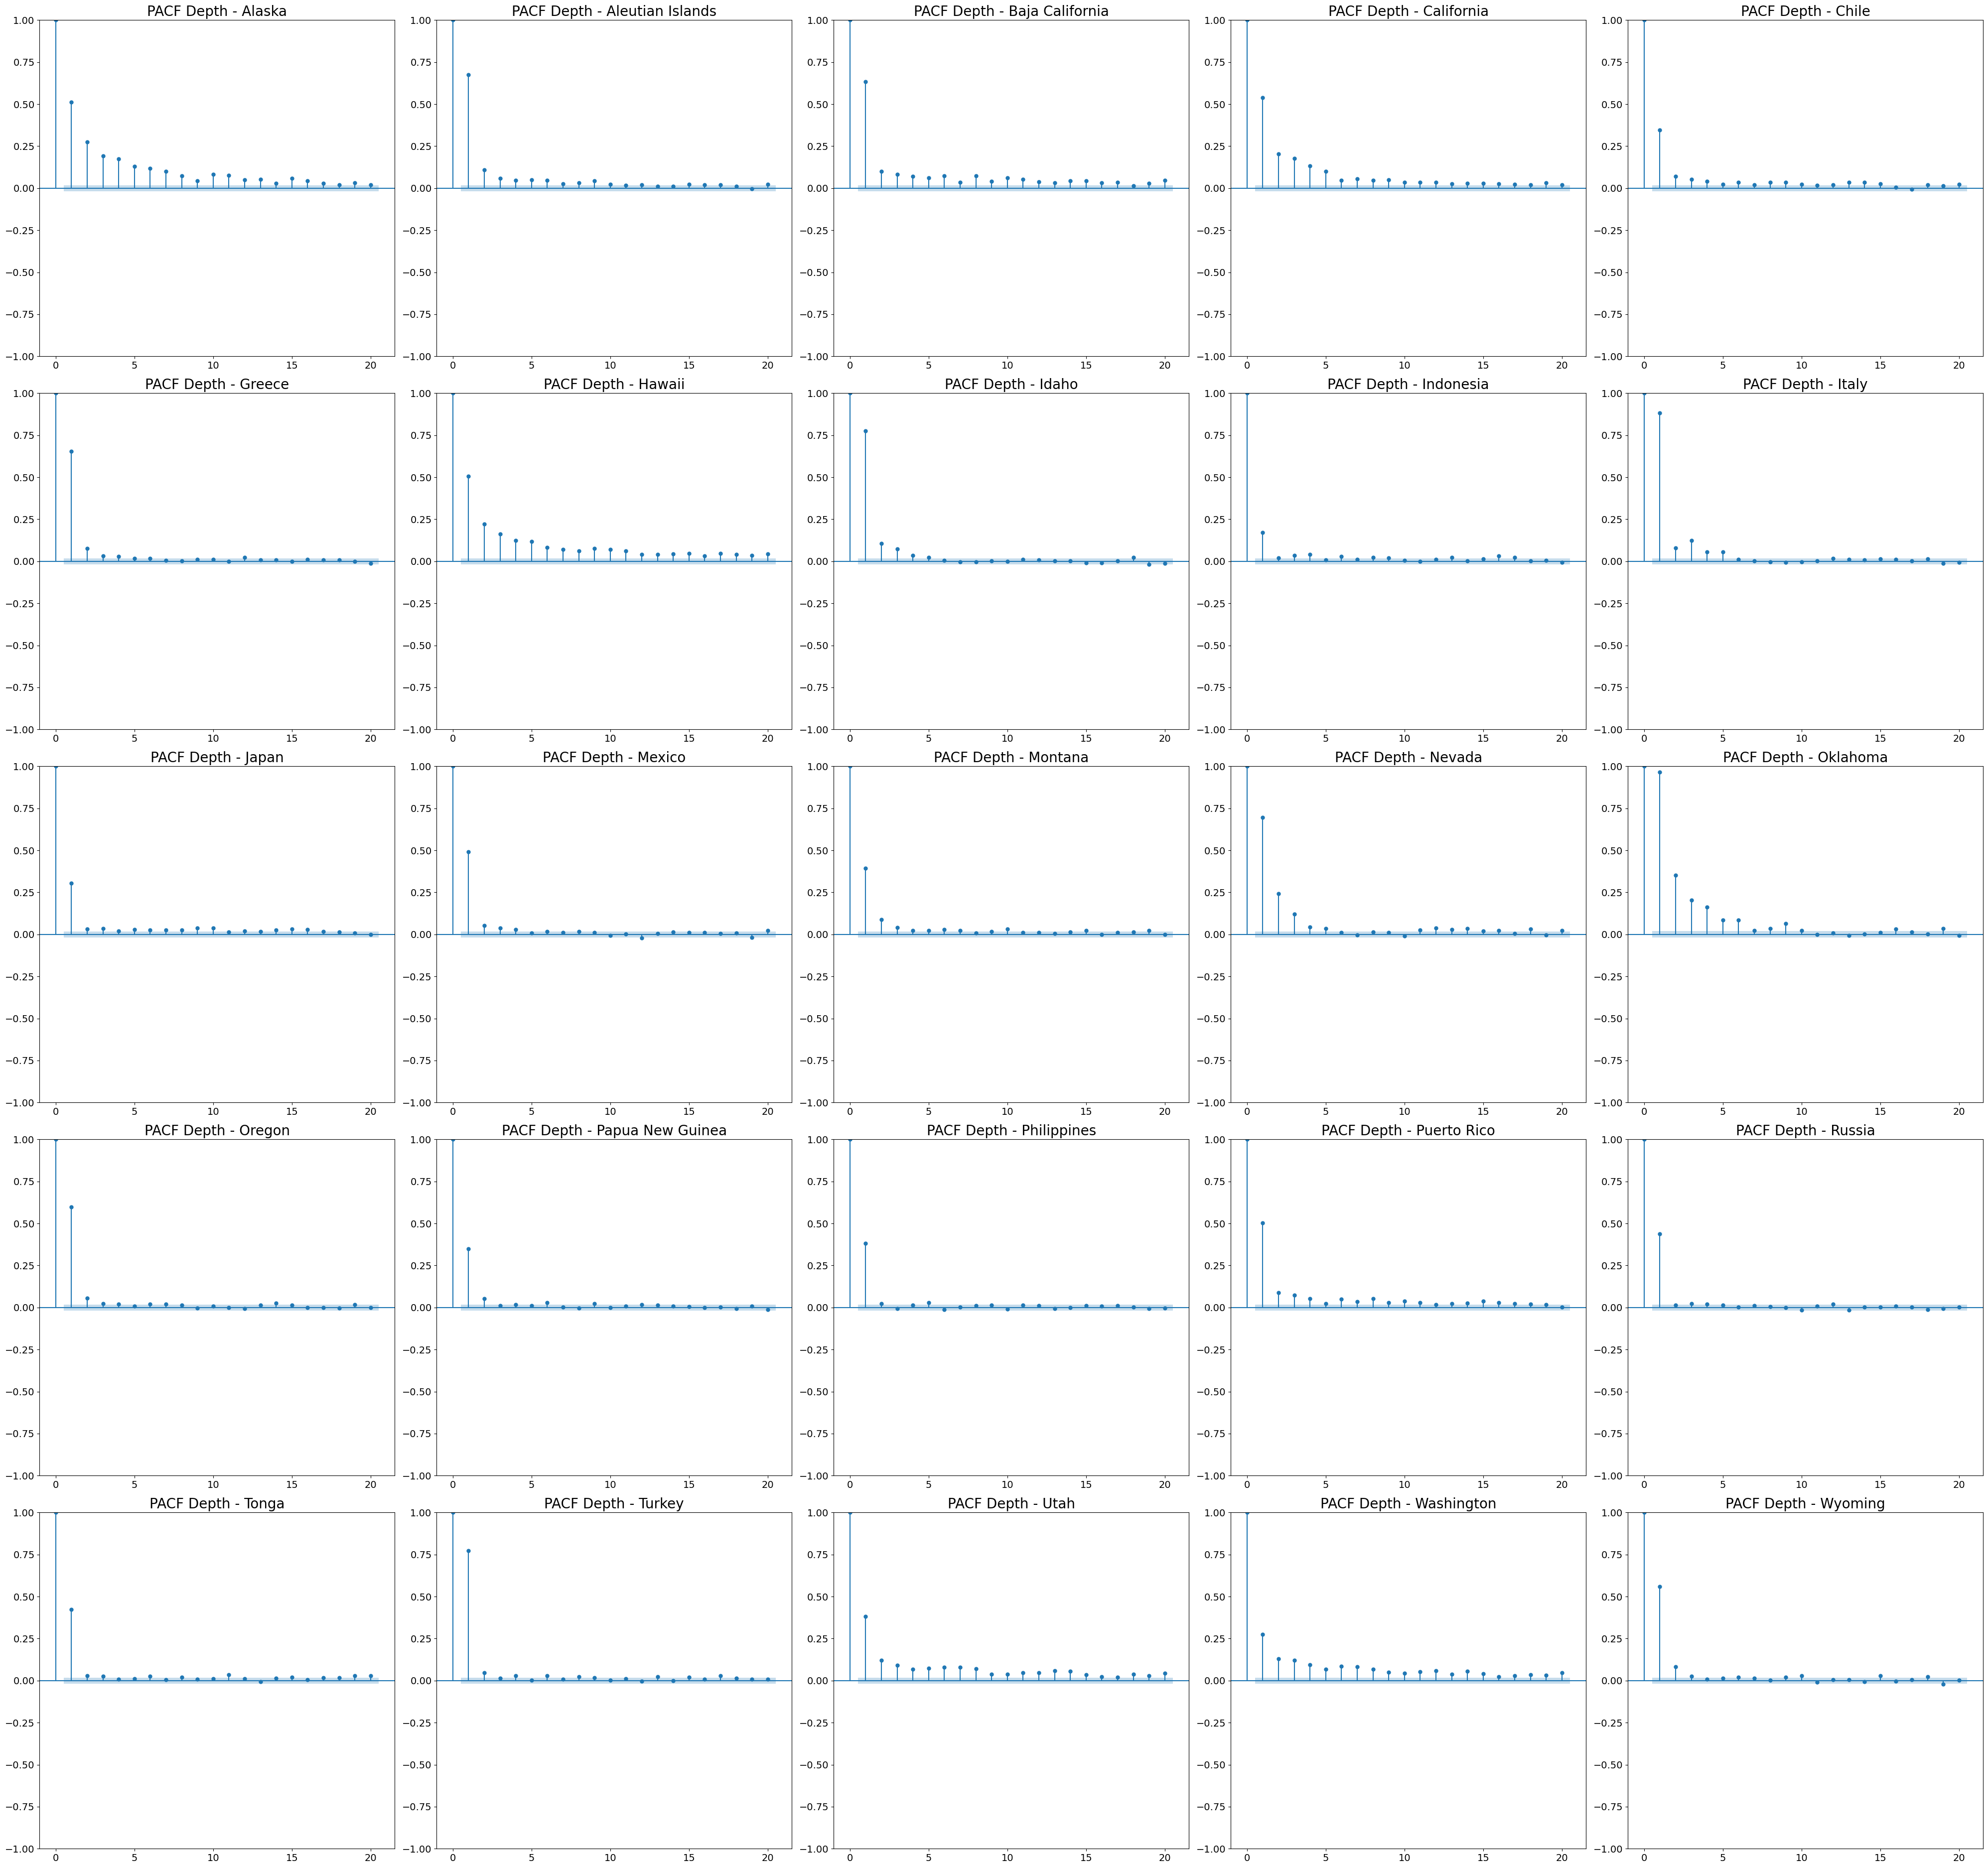
\includegraphics[scale=0.15]{img/depth-pacf-per-region.png}
    \captionsetup{format=hang}
    \caption{\label{fig:depth-pacf}Depth partial autocorrelation per region.}
\end{figure}

\begin{figure}[hbtp]
    \centering
    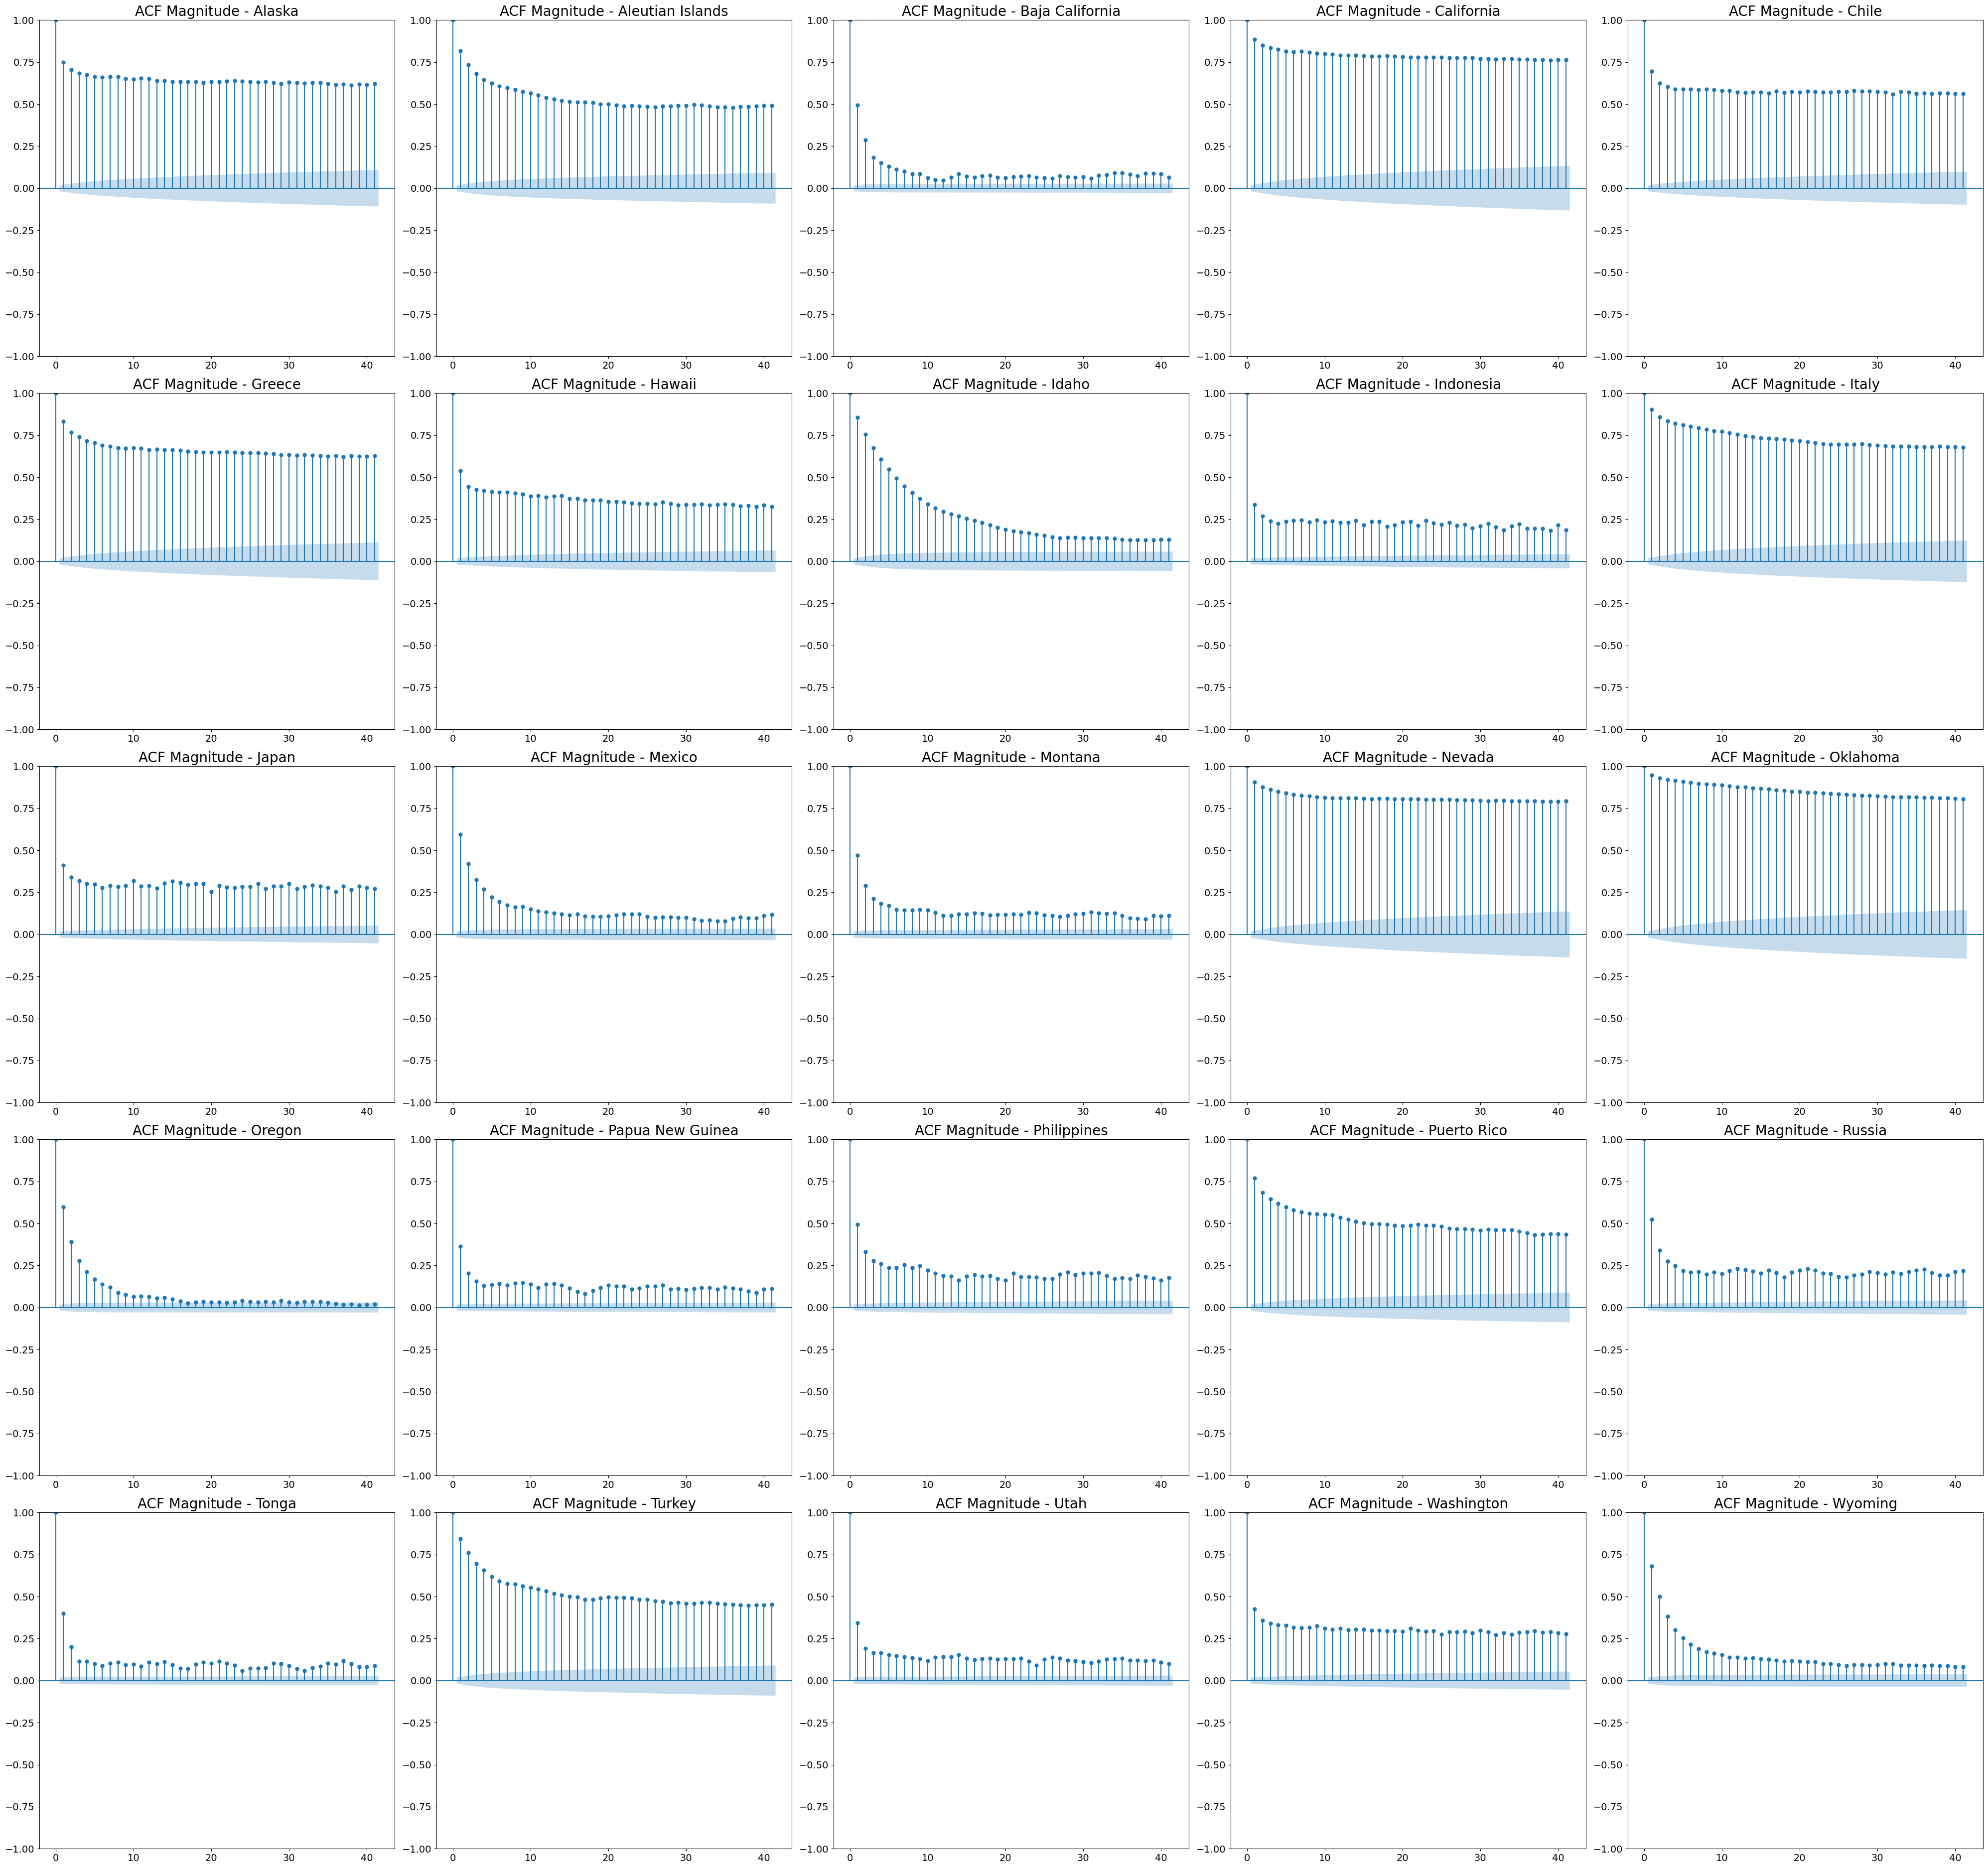
\includegraphics[scale=0.15]{img/magnitude-acf-per-region.png}
    \captionsetup{format=hang}
    \caption{\label{fig:mag-acf}Magnitude autocorrelation per region.}
\end{figure}

\begin{figure}[hbtp]
    \centering
    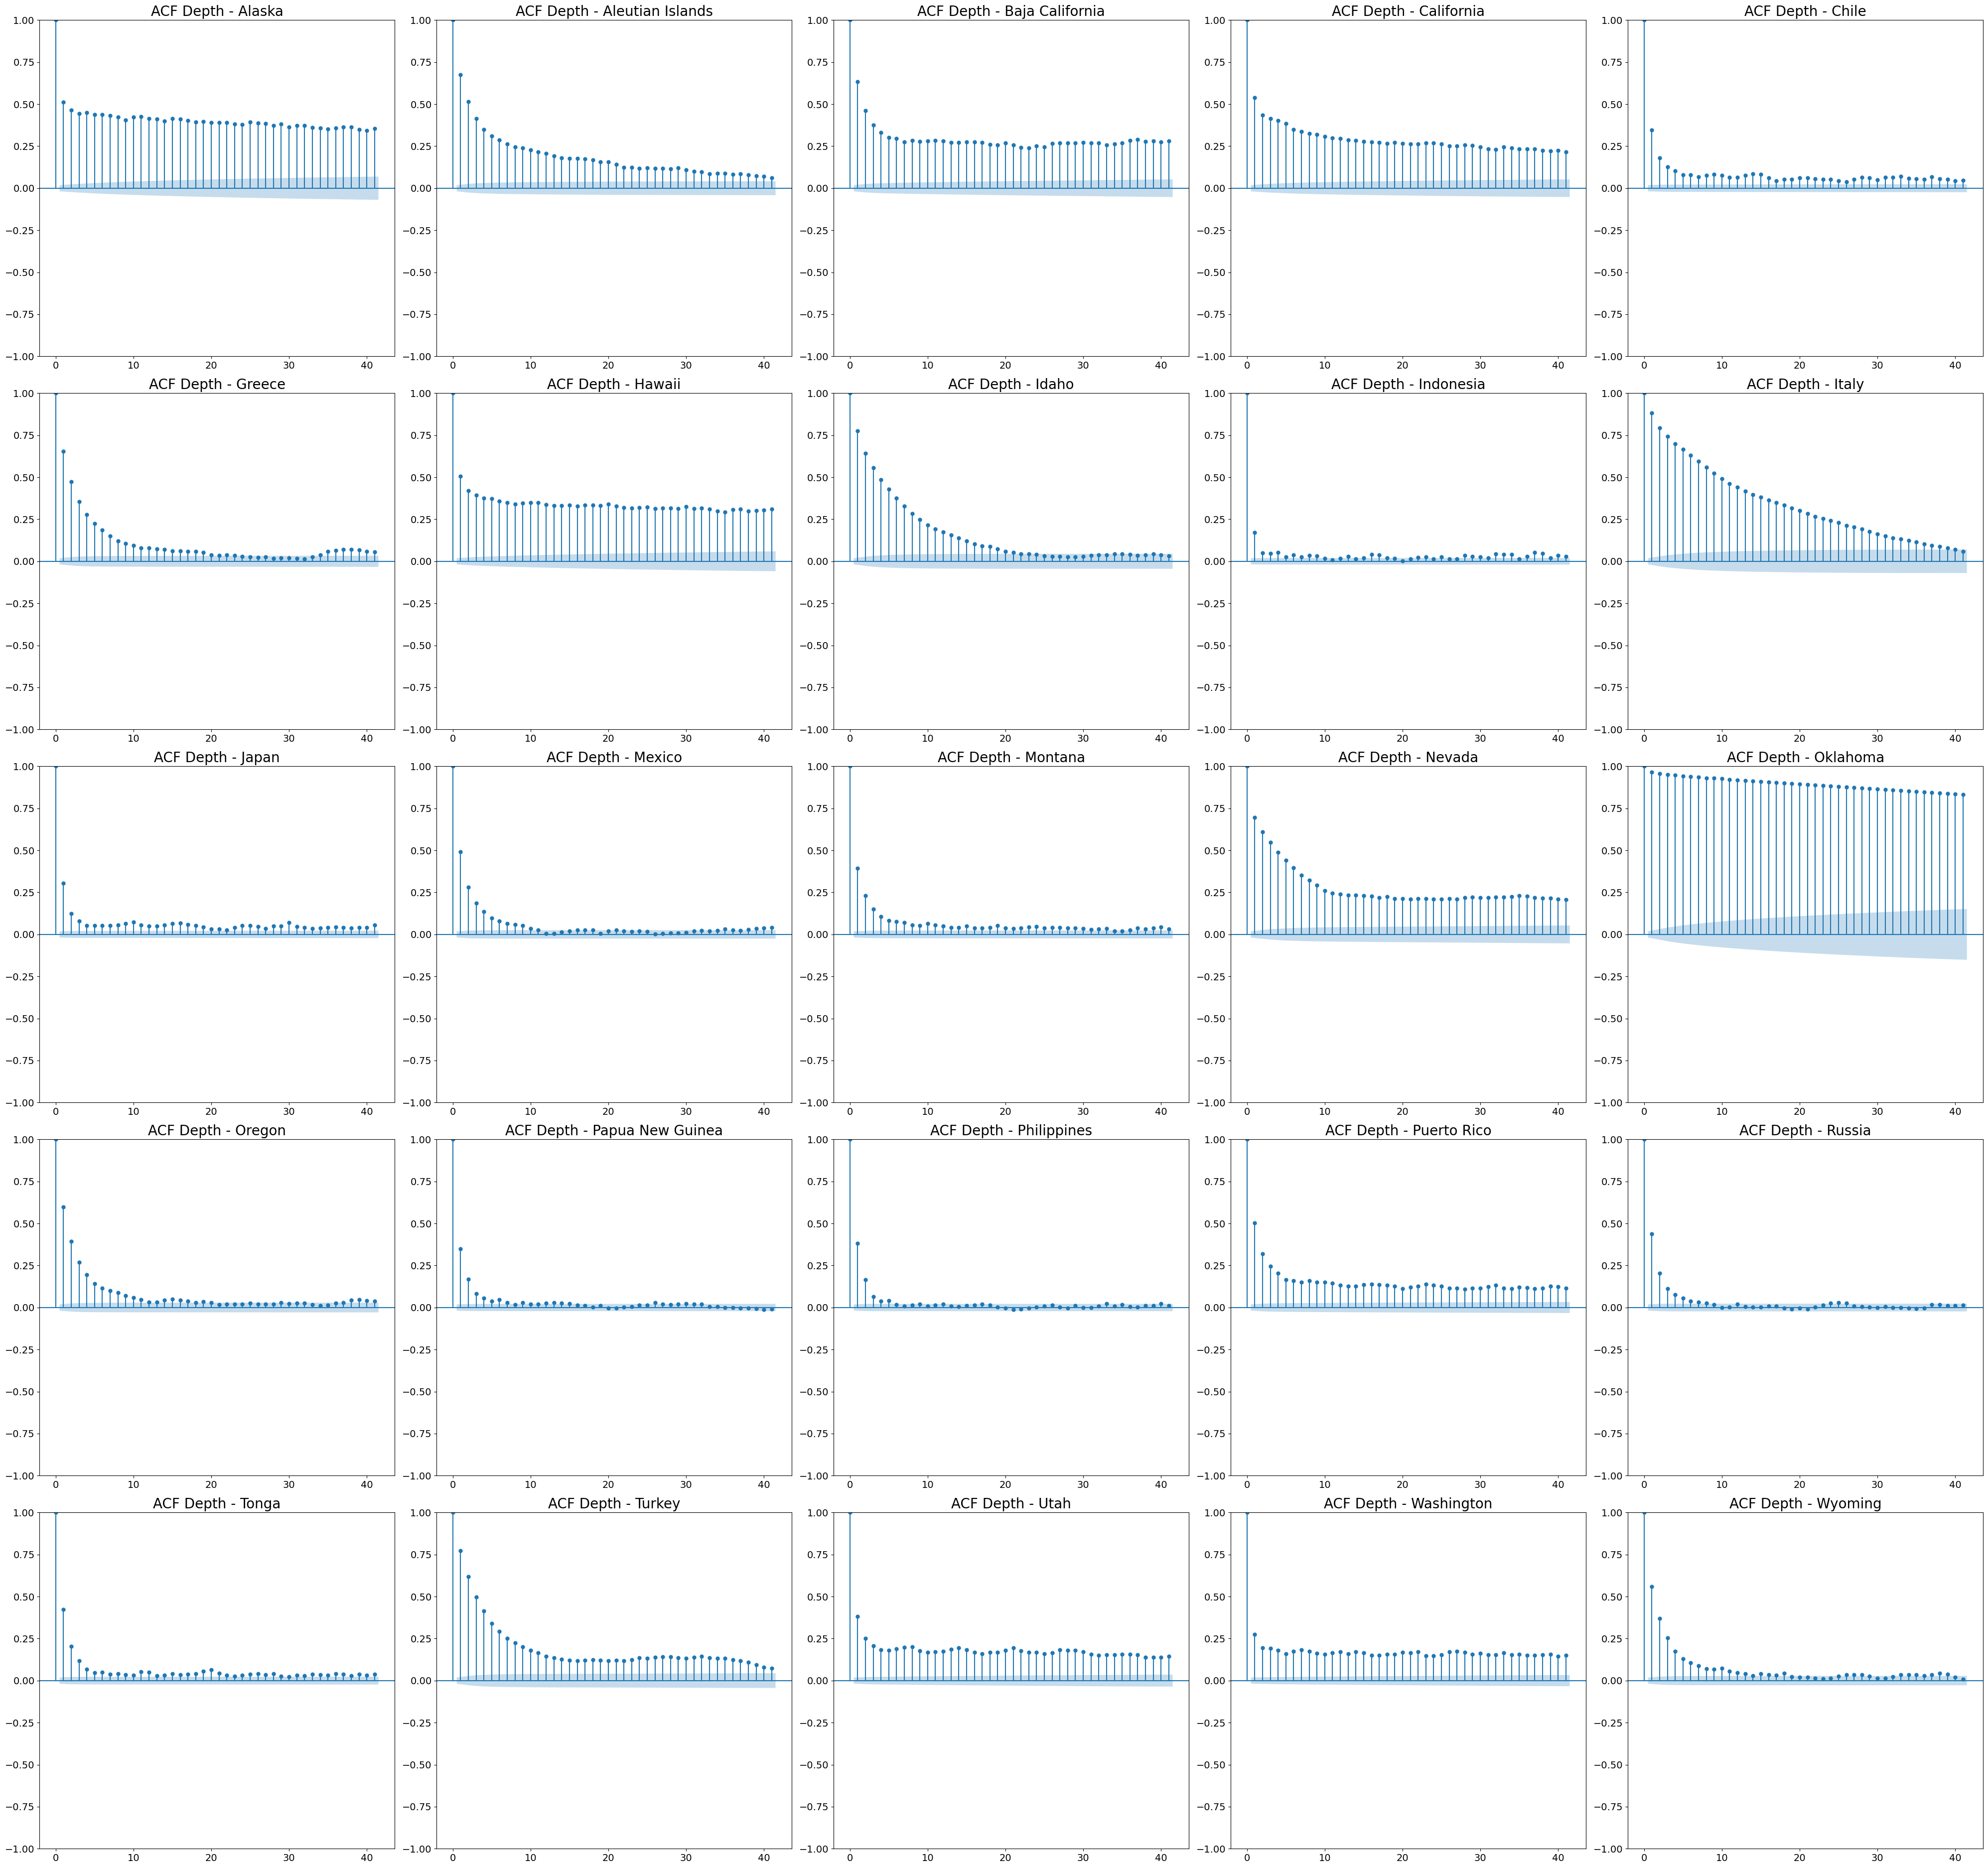
\includegraphics[scale=0.15]{img/depth-acf-per-region.png}
    \captionsetup{format=hang}
    \caption{\label{fig:depth-acf}Depth autocorrelation per region.}
\end{figure}

\begin{figure}[hbtp]
    \centering
    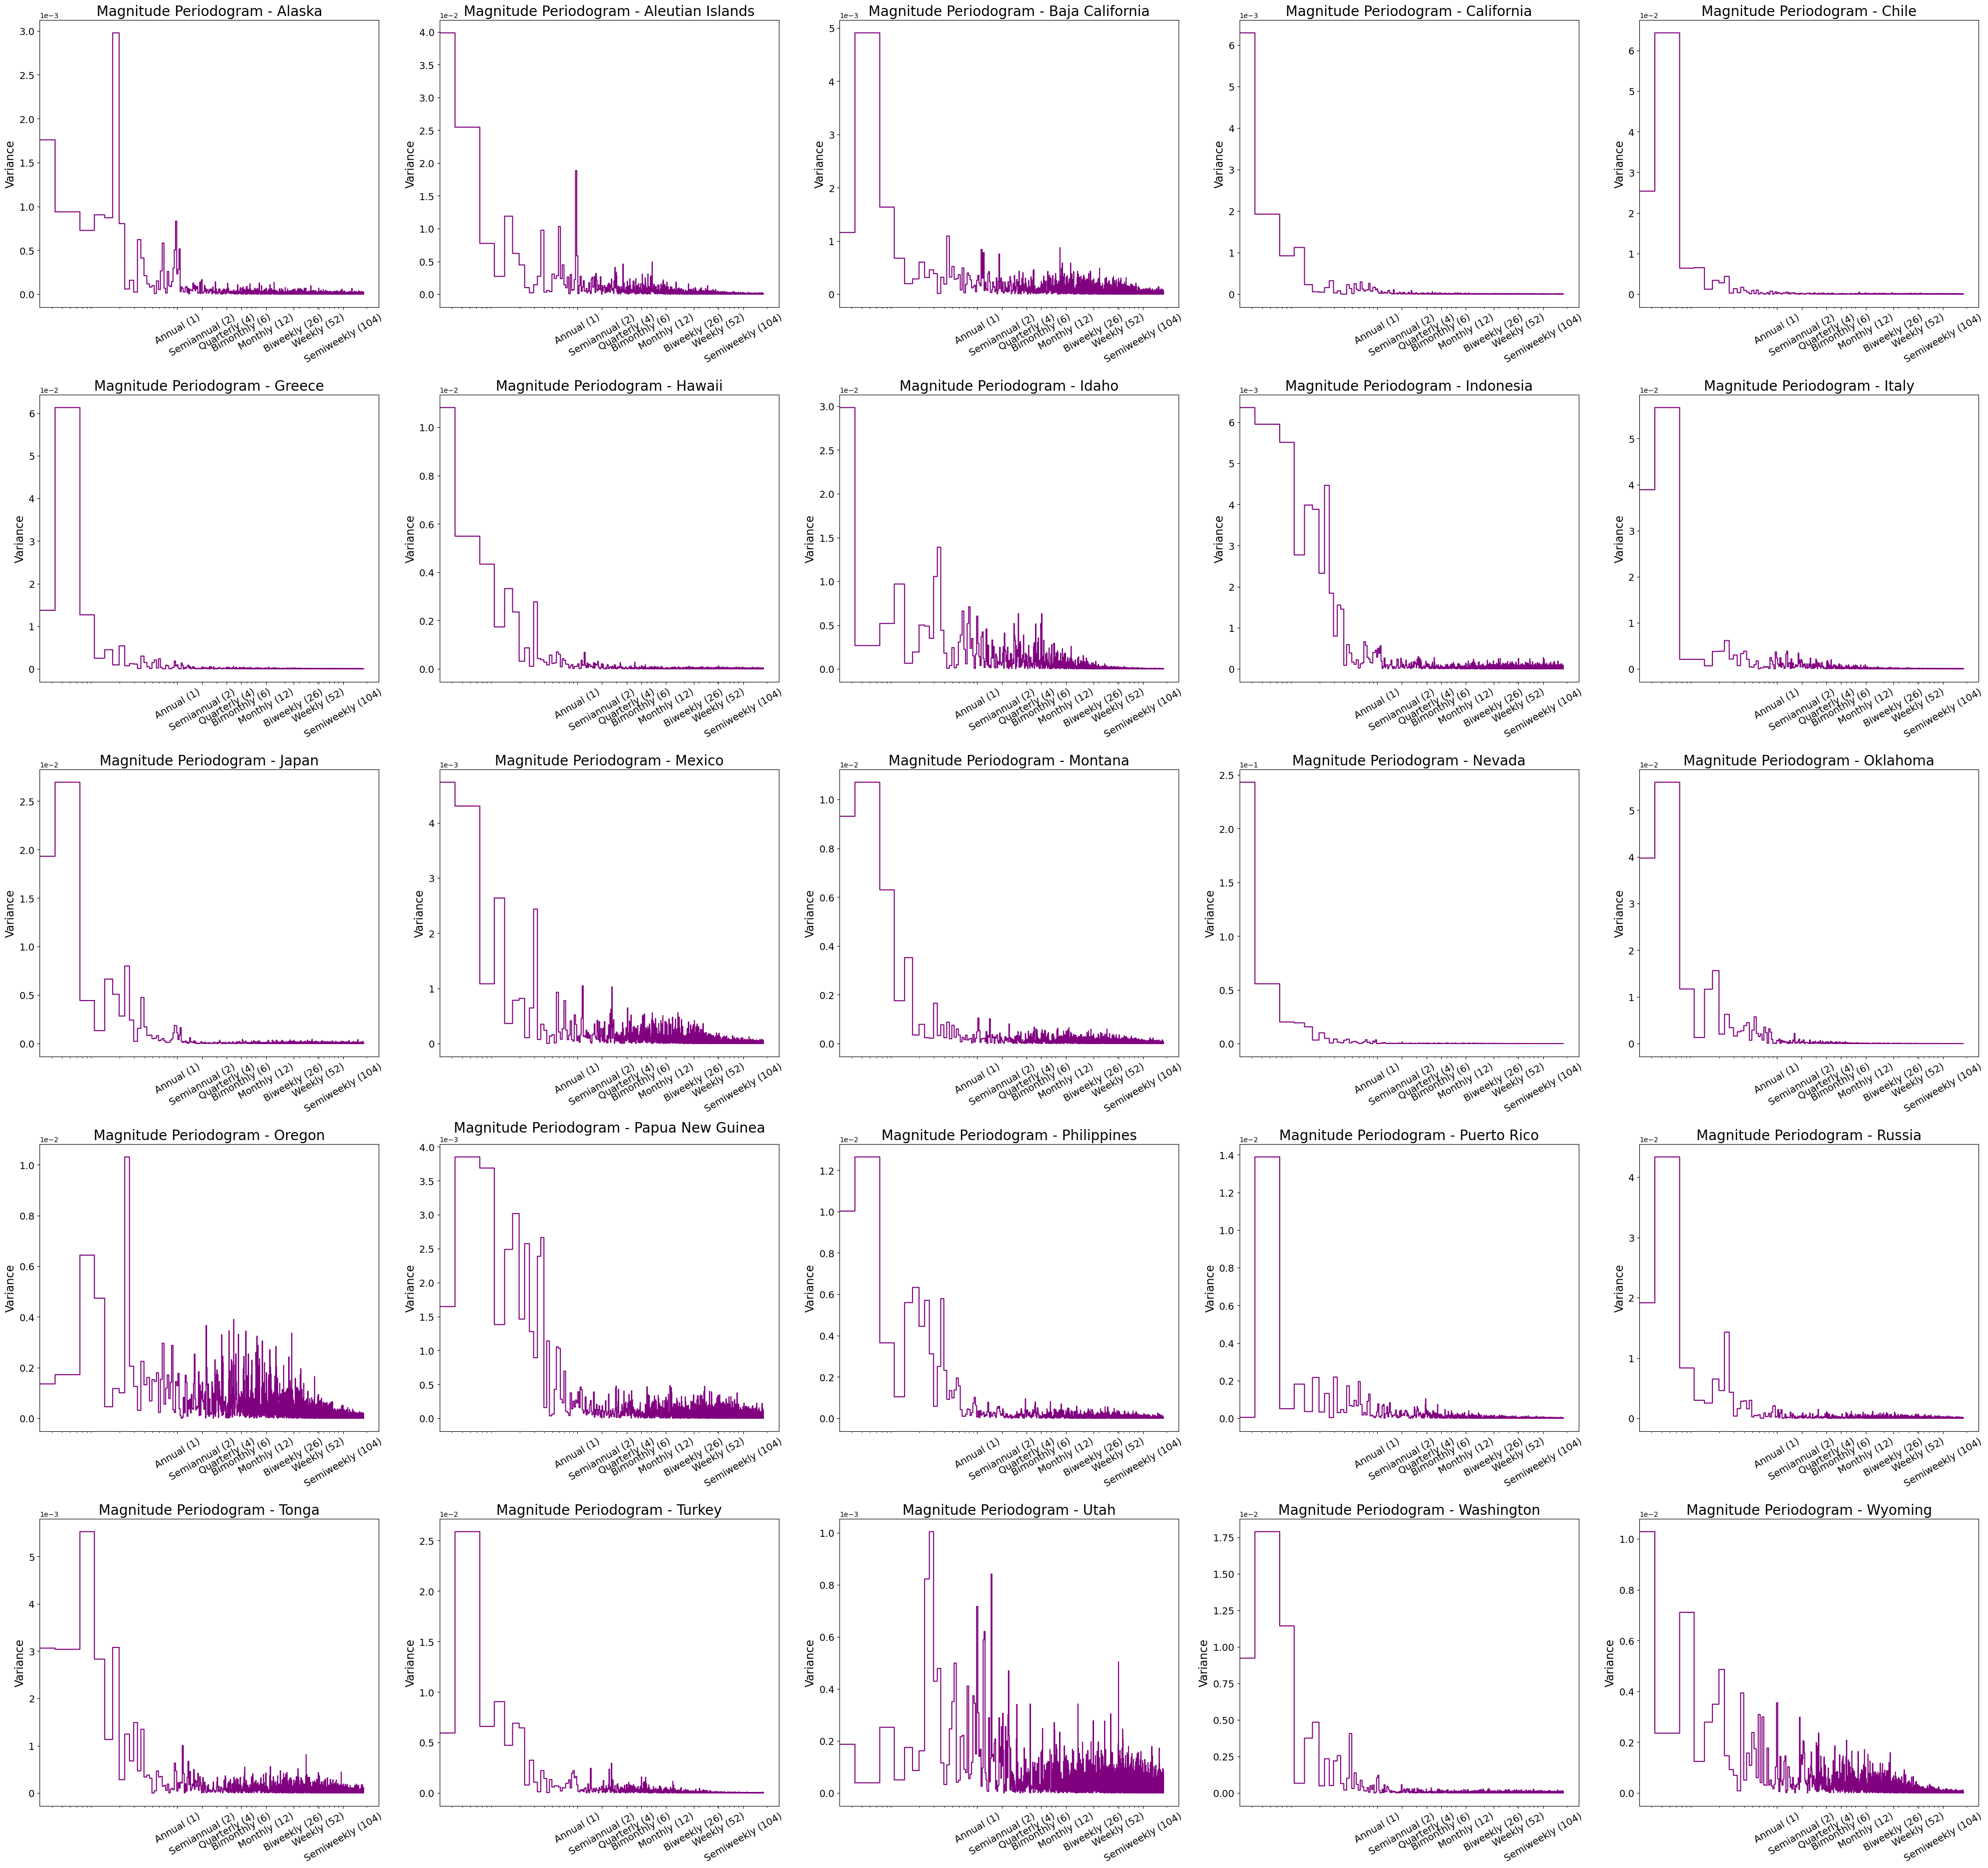
\includegraphics[scale=0.15]{img/magnitude-periodogram.png}
    \captionsetup{format=hang}
    \caption{\label{fig:mag-periodogram}Magnitude periodogram:
        spectral density of the magnitude as a function of frequency.}
\end{figure}

\begin{figure}[hbtp]
    \centering
    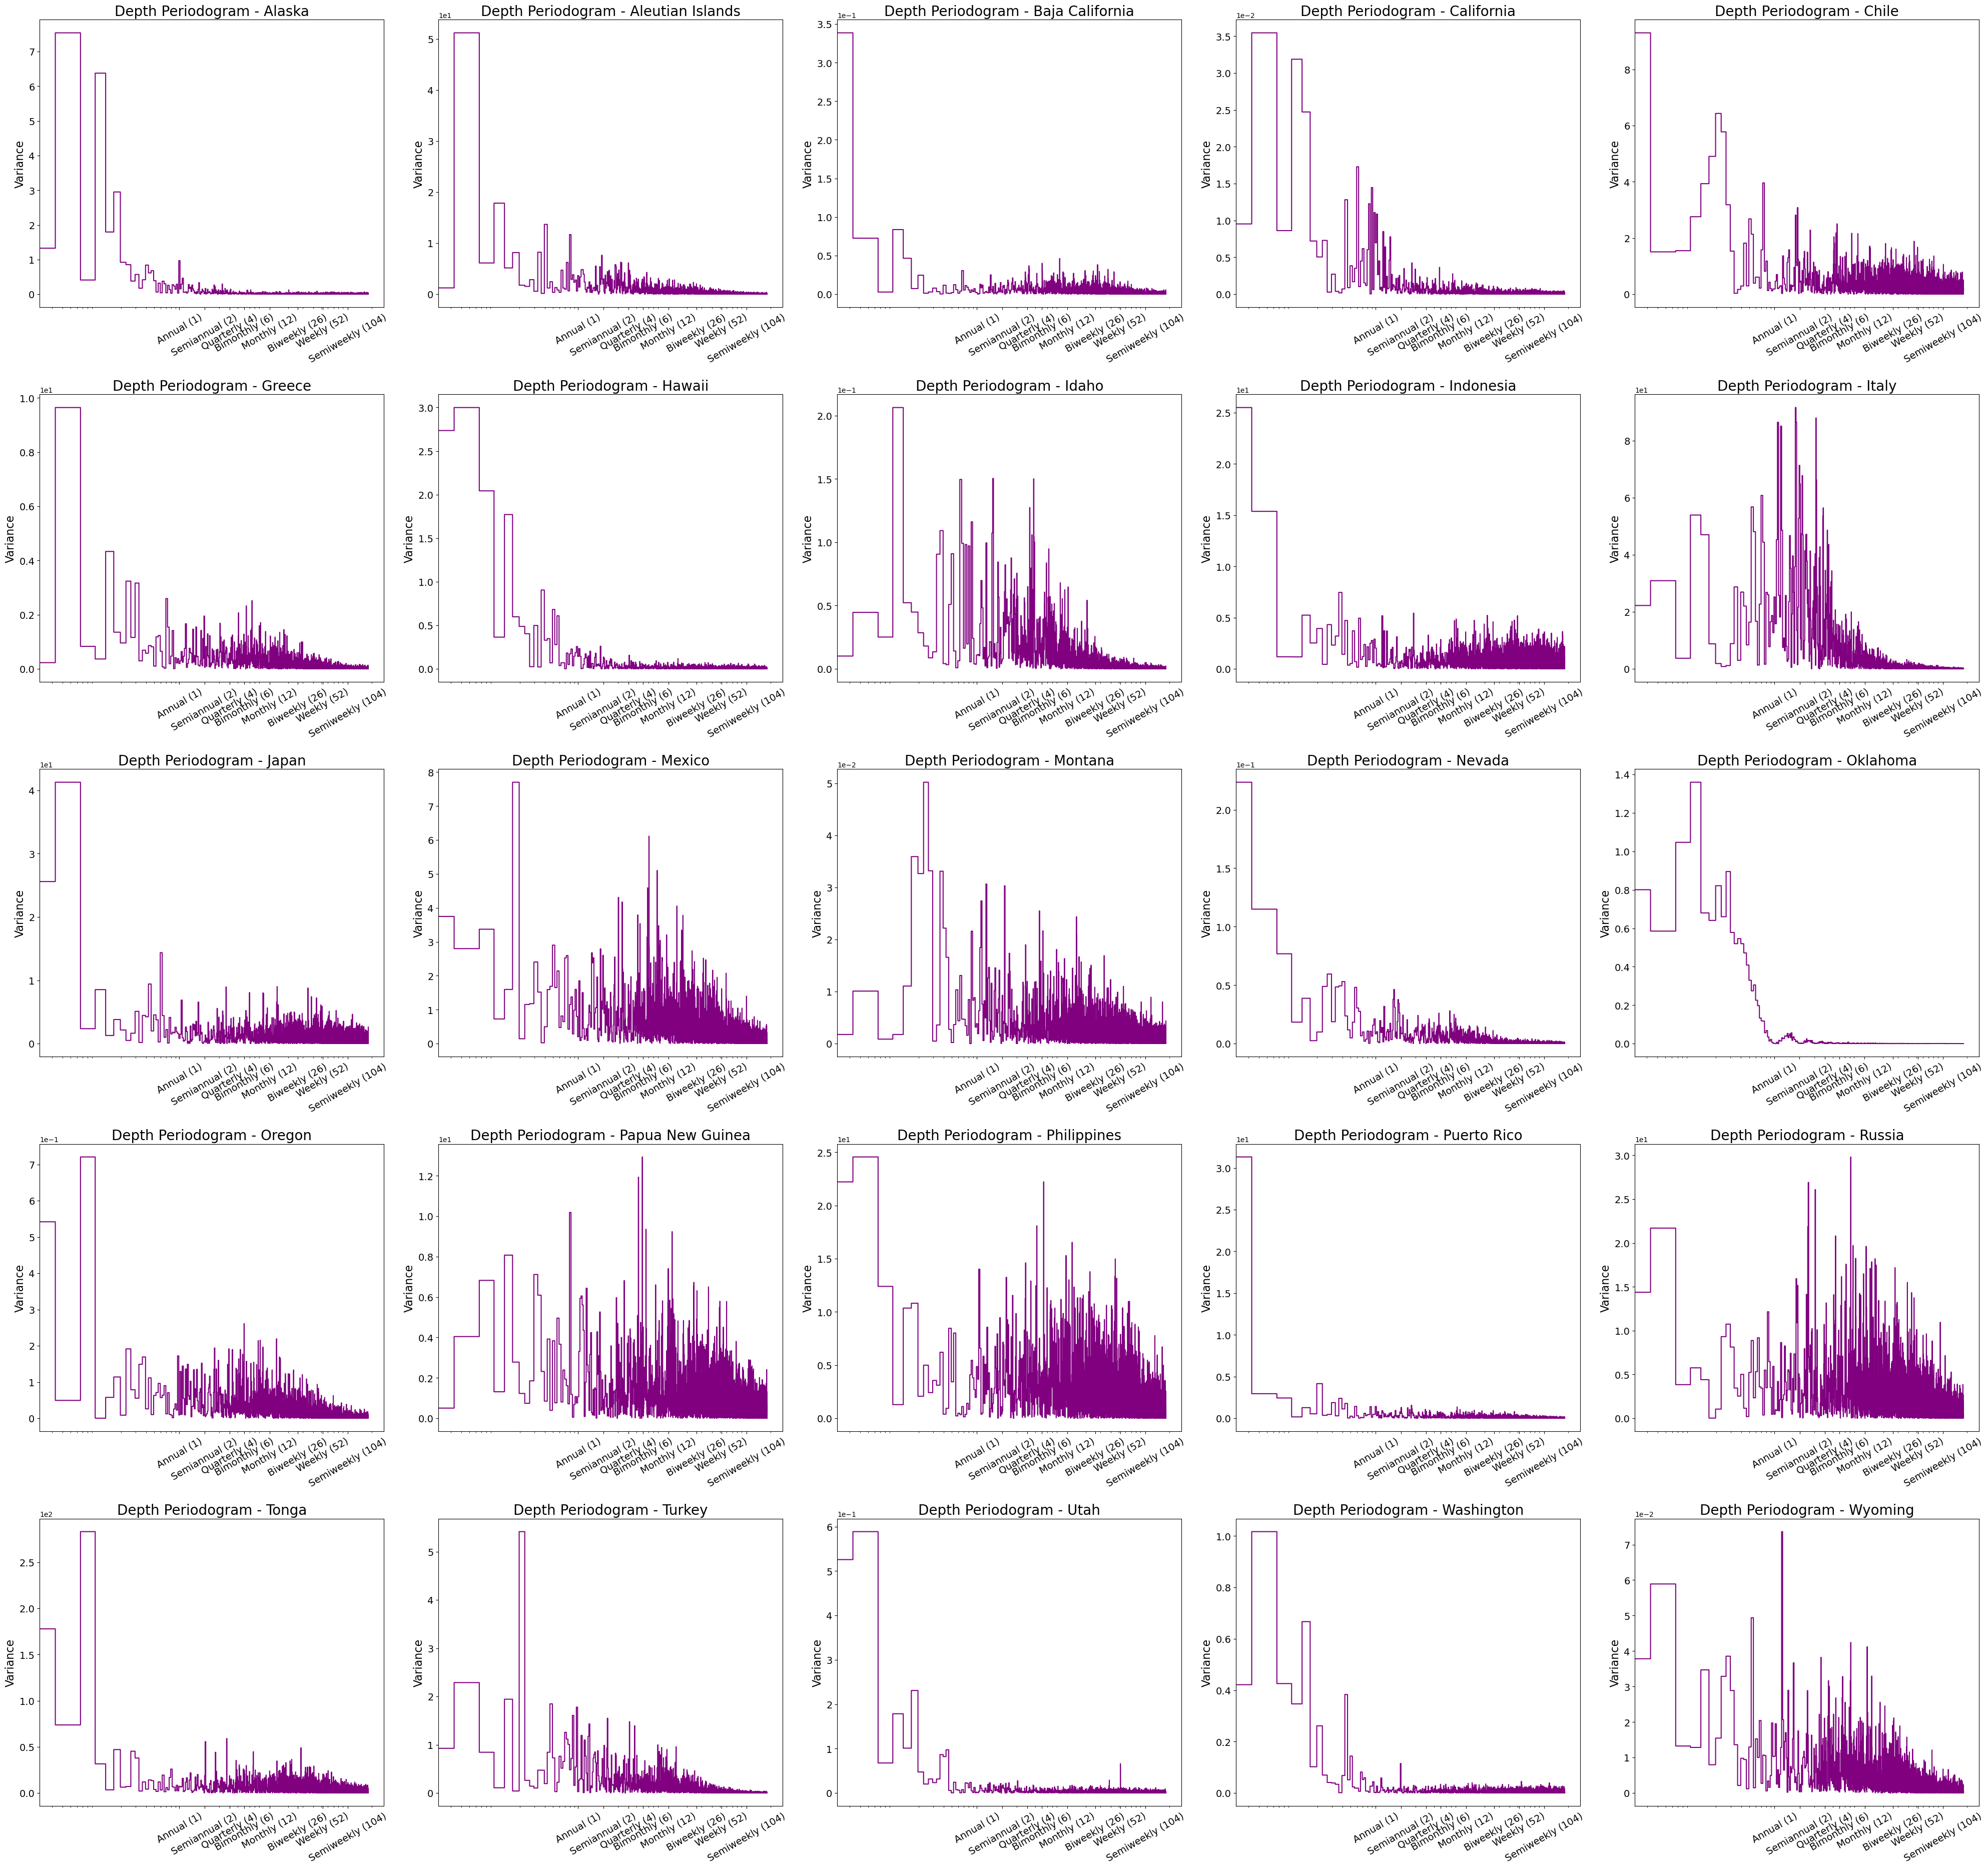
\includegraphics[scale=0.15]{img/depth-periodogram.png}
    \captionsetup{format=hang}
    \caption{\label{fig:depth-periodogram}Depth periodogram:
        spectral density of the depth as a function of frequency.}
\end{figure}

\begin{figure}[hbtp]
    \centering
    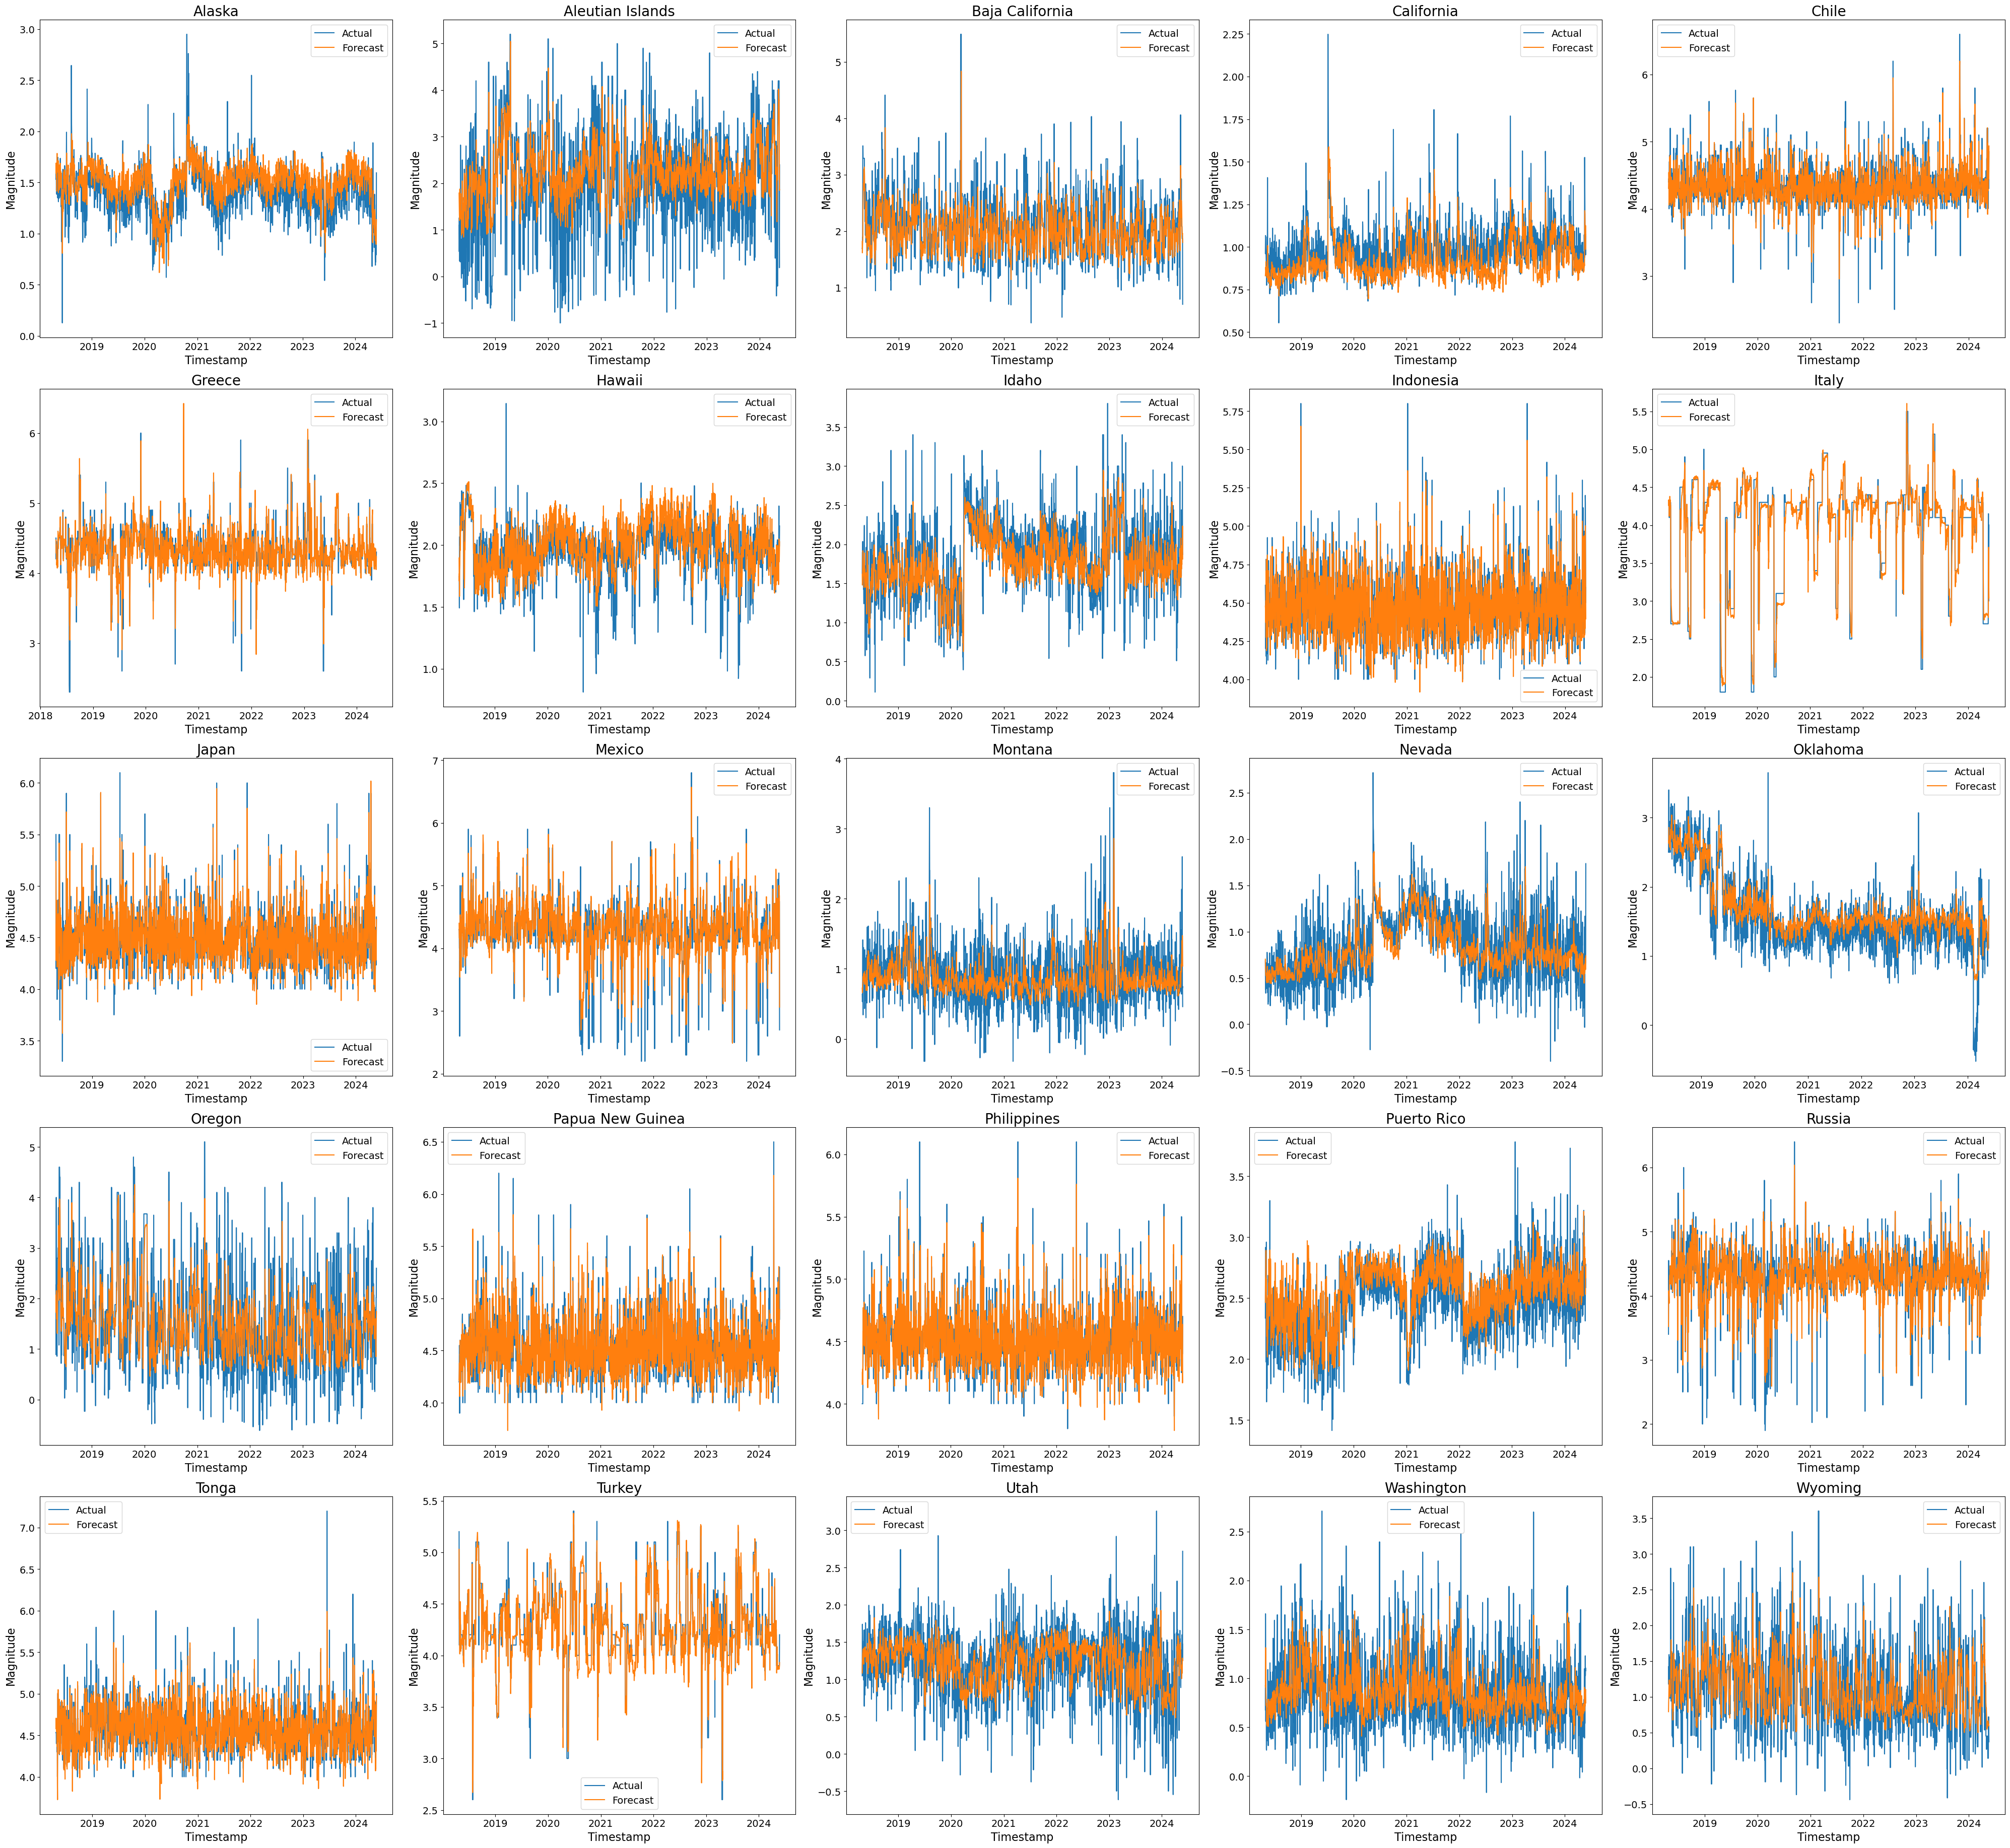
\includegraphics[scale=0.15]{img/magnitude-forecast-test-set.png}
    \captionsetup{format=hang}
    \caption{\label{fig:mag-forecast-full}Magnitude forecast per region on test set.}
\end{figure}

\begin{figure}[hbtp]
    \centering
    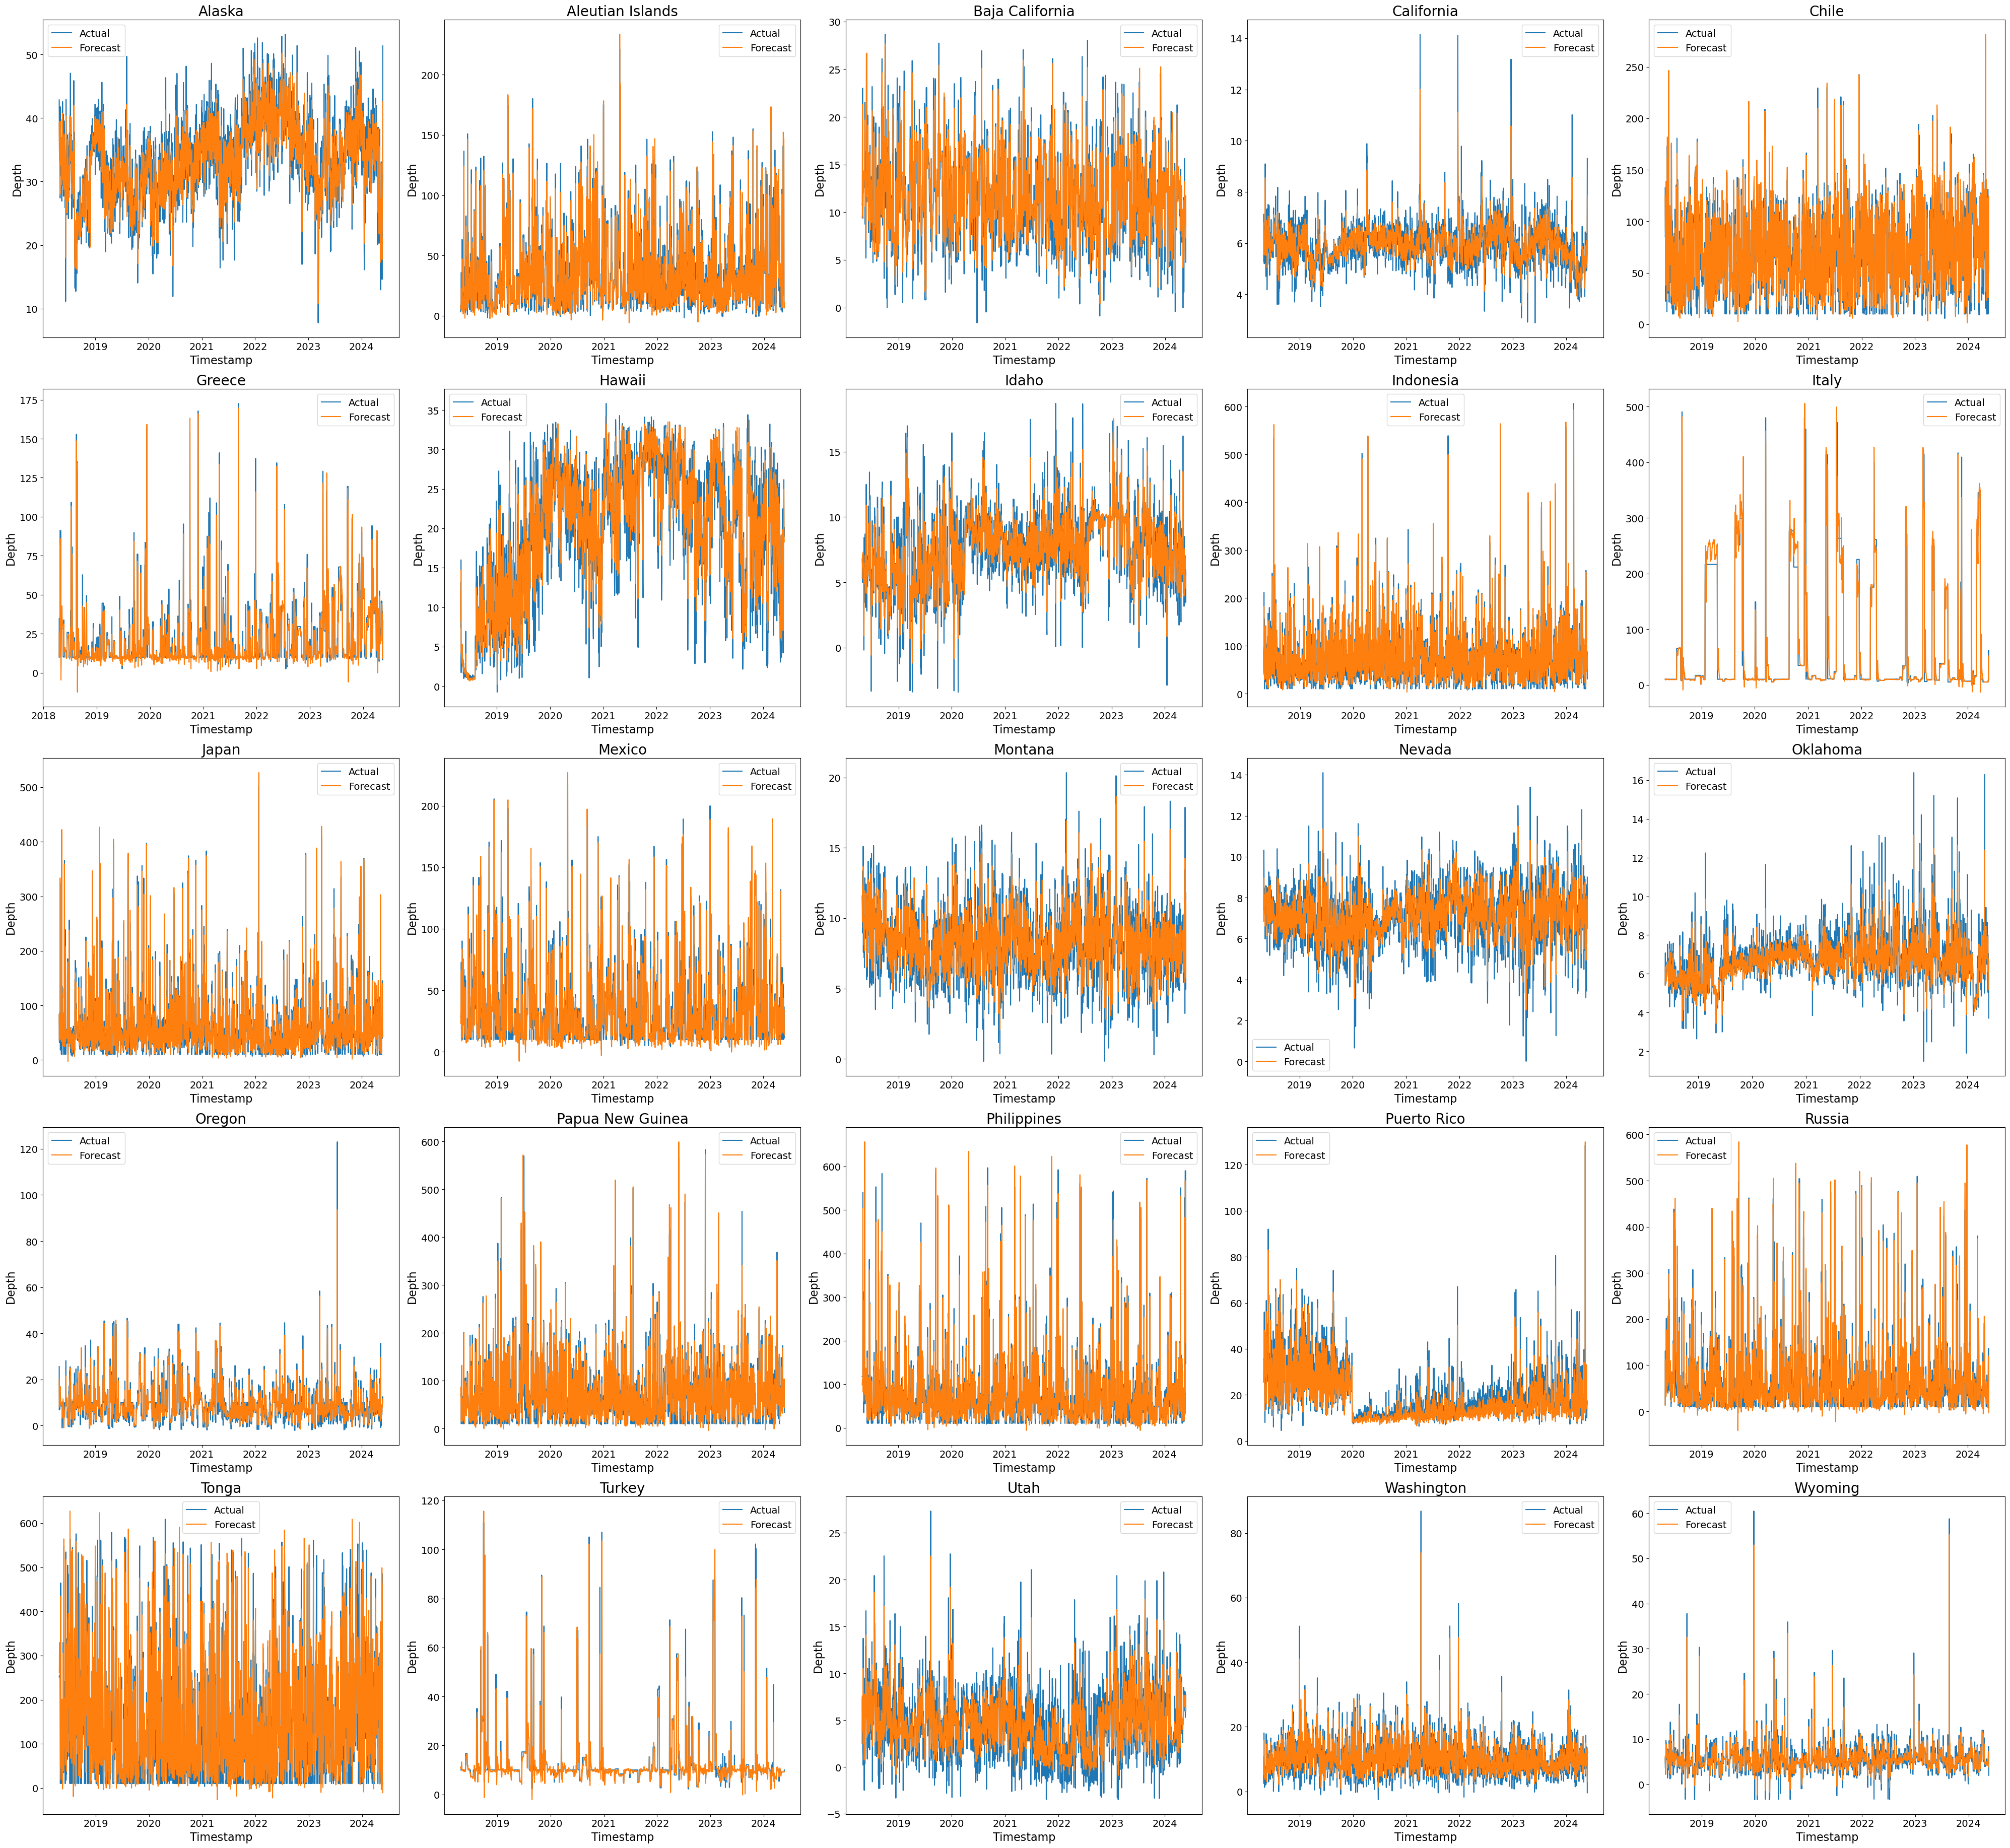
\includegraphics[scale=0.15]{img/depth-forecast-test-set.png}
    \captionsetup{format=hang}
    \caption{\label{fig:depth-forecast-full}Depth forecast per region on test set.}
\end{figure}